\documentclass[12pt, a4paper]{report}
\usepackage[utf8]{inputenc}
\usepackage[T1]{fontenc}
\usepackage[utf8]{inputenc}
\usepackage{geometry}
\usepackage{listings}
\usepackage{xcolor}
\usepackage[]{graphicx}
\usepackage[export]{adjustbox}
\usepackage{subcaption}
\makeatletter
\setlength{\@fptop}{0pt}
\makeatother

\definecolor{codegreen}{rgb}{0.26, 0.61, 0}
\definecolor{codegray}{rgb}{0.5,0.5,5}
\definecolor{codepurple}{rgb}{58,0,0.82}
\definecolor{backcolour}{rgb}{0.80, 0.81, 0.93}

\lstdefinestyle{mystyle}{
    backgroundcolor=\color{backcolour},   
    commentstyle=\color{codegreen},
    keywordstyle=\color{magenta},
    numberstyle=\tiny\color{codegray},
    stringstyle=\color{codepurple},
    basicstyle=\ttfamily\footnotesize,
    breakatwhitespace=false,         
    breaklines=true,                 
    captionpos=b,                    
    keepspaces=true,                 
    numbers=left,                    
    numbersep=5pt,                  
    showspaces=false,                
    showstringspaces=false,
    showtabs=false,                  
    tabsize=2
}

\lstset{style=mystyle}


\title{\textbf{EE2703: Applied Programming Lab\\Assignment 7\\
}}


\author{Devaganthan S S\\ EE19B018}
\date{\today}
\begin{document}

\maketitle


\section{Abstract}
This assignment aims to focus on two powerful capabilities of python:
\begin{itemize}
  \item Symbolic Algebra
  \item Analysis of Circuits Using Laplace Transforms
\end{itemize}

\section{Introduction}
Python can be used to solve Circuits, get Transfer Functions, by formulating Matrices. In this assignment, we try to find Output to a High and Low pass Filters, with majorly using sympy functions. The idea is to form expressions of Transfer Functions or Output, with help of the \textbf{‘symbol()’}  function, and then convert it into an LTI system. With the help of \textbf{‘lsim()’} or \textbf{‘step()’} functions, we can find the output response.
\section{Results and Implementation}
\subsection{Step Response of LPF:}
We first find the expression for the transfer function of the LPF, assuming the input(Vi) as 1. Then with the help of the \textbf{‘step()’} function, we find the step response of the LPF. The below code accomplishes the above tasks and plots the Step Response.
\noindent
\lstinputlisting[language = python]{code1.py}
\begin{figure}[h!]
    \centering
    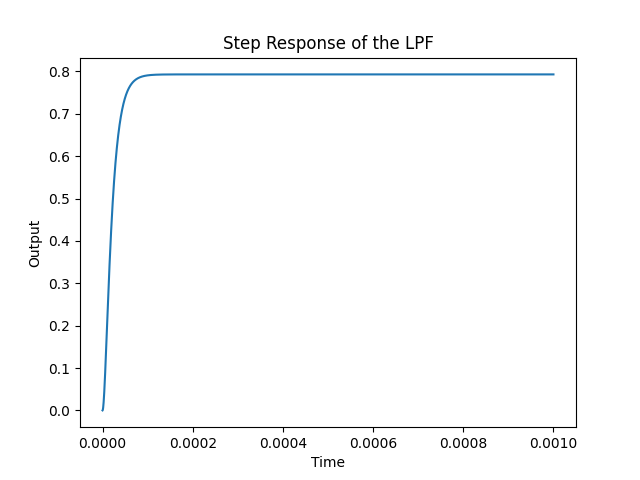
\includegraphics[scale=0.75]{fig1.png} 
    \caption{}
    \label{fig:my_label}
\end{figure}
\vspace{100mm}
\subsection{Output to the Given Signal:}
For the given input, $v_i(t) = (sin(2000\pi t)+cos(2.10^6\pi t))u_o(t)$, the output can be found using the \textbf{‘lsim()’} function. The transfer function H is obtained from the previous part. The below code finds the output and plots the same. From the plot, we can see that the output has only low frequency, (2000\pi sine).



\lstinputlisting[language = python]{code2.py}
\begin{figure}[h!]
    \centering
    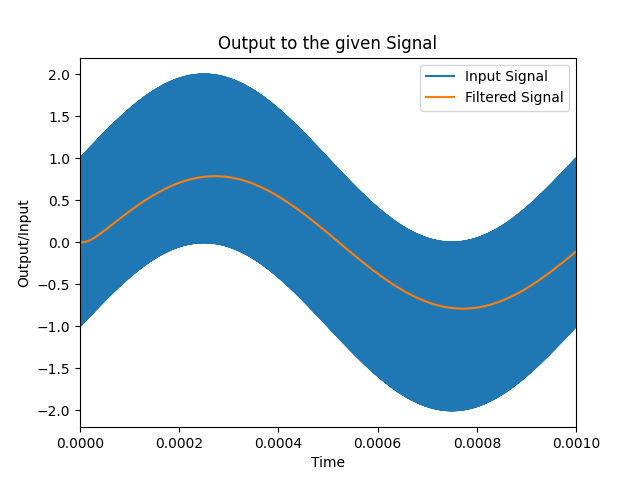
\includegraphics[scale=0.75]{fig2.png} 
    \caption{}
    \label{fig:my_label}
\end{figure}
\vspace{100mm}
\subsection{Magnitude Plot of HPF}
Adopting the same procedure as before for the LPF, we find the Transfer function for the HPF. We plot the Magnitude vs Phase Plot. The below code accomplishes the above tasks.
\noindent
\lstinputlisting[language = python]{code3.py}
\vspace{100mm}
\begin{figure}[h!]
    \centering
    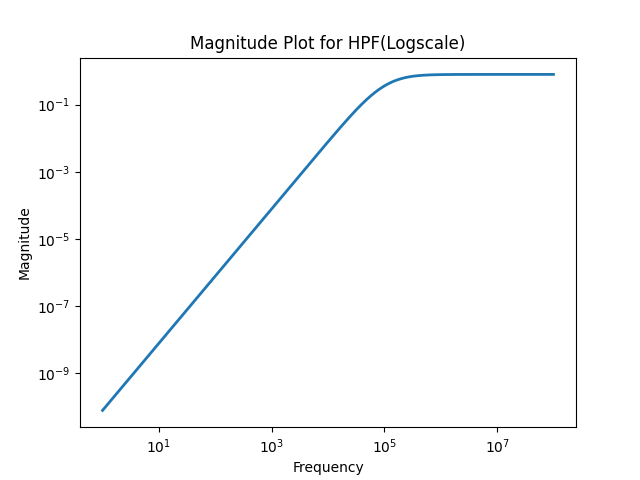
\includegraphics[scale=0.75]{fig3.png} 
    \caption{}
    \label{fig:my_label}
\end{figure}
\subsection{Output for a Damped Sinusoid for the HPF}
Using the Transfer Function from the previous part and using the function \textbf{‘lsim()’} we can find the response to the Damped Sinusoid for the HPF. The below code computes the output and plots the same. From the plots, we can see that the high frequencies amplitude have been reduced a bit, but whereas the low frequencies are completely suppressed.
\noindent
\lstinputlisting[language = python]{code4.py}
\begin{figure}[h!]
    \centering
    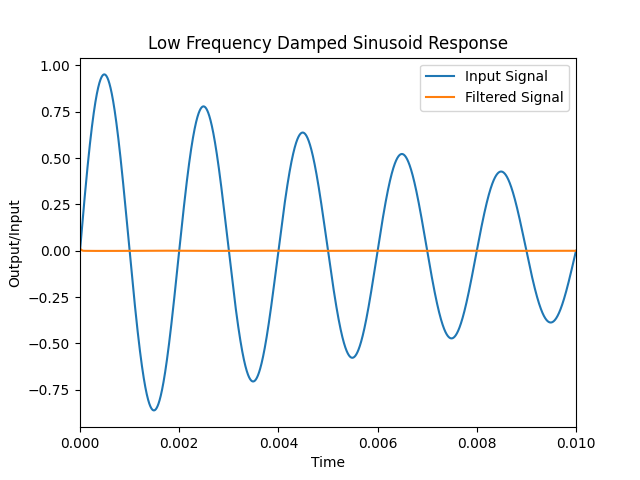
\includegraphics[scale=0.75]{fig4.png} 
    \caption{}
    \label{fig:my_label}
\end{figure}
\vspace{100mm}
\begin{figure}[h!]
    \centering
    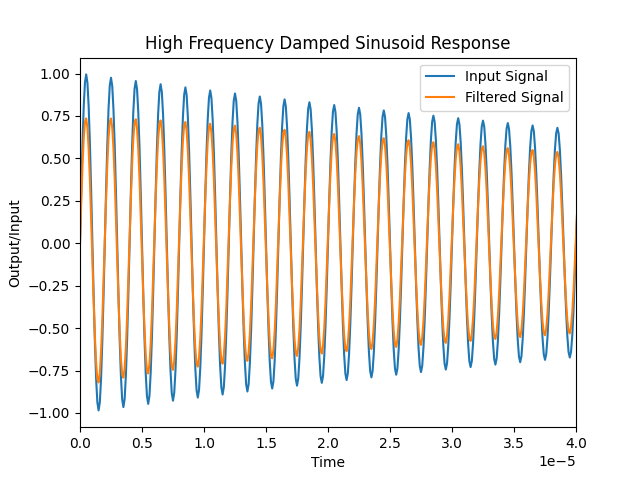
\includegraphics[scale=0.75]{fig5.png} 
    \caption{}
    \label{fig:my_label}
\end{figure}
\subsection{Step Response for the HPF:}
The same procedure as the LPF case has been followed to find the step response. The below computes the step response and plots the same.
\vspace{100mm}
\noindent
\lstinputlisting[language = python]{code5.py}
\begin{figure}[h!]
    \centering
    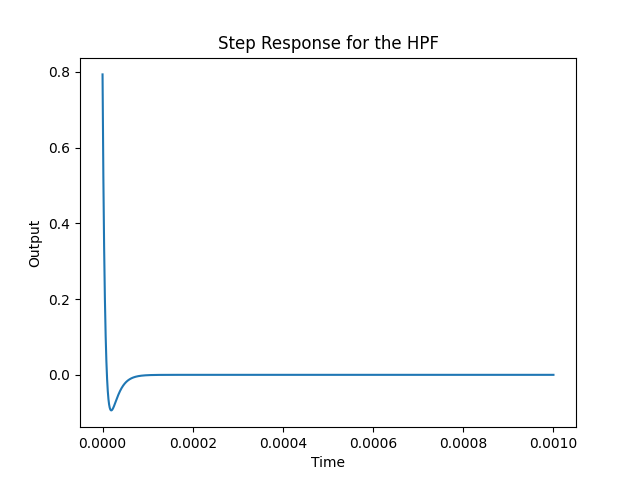
\includegraphics[scale=0.75]{fig6.png} 
    \caption{}
    \label{fig:my_label}
\end{figure}

\section{Conclusion}
Symbolic Algebra and Signal toolbox are powerful tools that help to solve Complex Circuit Problems. Laplace Transform Analysis of circuits can be effectively done in python.


\end{document}

